In this section, we explain in detail our encoding of the UC security definition into Nomos-UC.
Recall from Section~\ref{sec:background} that the UC security definition $\F_1 \xrightarrow{\pi} \F_2$ says we can realize some desired application $\F_2$ with a protocol $\pi$ that uses $\F_1$.
More generally, we define UC realization in terms of an indistinguishability relation between two experiments: the real-world featuring the execution of $\pi$ with $\F_1$, and an ideal-world execution of $\F_2$ with an ideal protocol $\idealP$ that relays inputs/outputs directly to/from $\F_2$.%
\footnote{This ideal protocol $\idealP$ is also the identity, since we can easily show $\F \xrightarrow{\idealP} \F$ for any functionality $\F$.}
Below, we introduce how the UC experiment is defined in NomosUC, and then provide a composition operator $\circ$ for protocols and simulators that satisfies Theorem~\ref{thm:singlecomp}.

\subsection{The UC Experiment}
%The UC experiment is an execution of protocol parties and an ideal functionality, reacting to input by an adversary \A or the environment \Z.
The type definition of \inline{execUC} is straightforward \todo{once we have clarity on the intro and type system section length we can include the typedef of here}. 
It is parameterized by at least one virtual token type to allow for sandboxing of other processes (usually by the adversary or environment) and message types specified by the protocolin question. 
Its only functional parameters are the security parameter $k$ and a random bit string $r$. 
An example typedef for the commitment example is in Figure~\ref{fig:execuc} where there are no virtual token types as the simulator doesn't perform any sandboxing.
Its type \m{execout} is defined as follows:
{\centering
\parbox{0cm}{
\begin{tabbing} 
 $\m{execout}[a] = \textcolor{red}{\getpot^n} \echoice{\mb{exec}: $\=$ \ichoice{ out: Bit \product 1}}$ 
 \end{tabbing}}
}

\begin{figure*}
\begin{lstlisting}[basicstyle=\footnotesize\BeraMonottFamily, mathescape, frame=single]
$\nproc$ execUC[K][p2f,f2p][z2p,p2z][a2p,p2a][f2a,a2f]{p2fn,f2pn}{z2pn,p2zn}{a2pn,p2an}{f2an,a2fn}{n}: 
  (k: Int), (rng: [Bit]) |- ($\$$d: execout)
\end{lstlisting}
\caption{Type definition for \m{execUC} with no virtual tokens.}
\label{fig:execuc}
\end{figure*}

The message types are used the providerless channels of of the main processs. For example, the communicator between \Z and \A is instantiated as
\begin{lstlisting}[basicstyle=\footnotesize\BeraMonottFamily, mathescape]
#z_to_a $\leftarrow$ channel_init[$\tp{K}$][$\tp{z2a}$]{$\tp{z2an}$}
#a_to_z $\leftarrow$ channel_init[$\tp{K}$][$\tp{a2z}$]{$\tp{a2zn}$}
\end{lstlisting}
where the type of \inline{#z_to_a} is given in Section~\ref{subsec:communicators} and its type parameters like $\tp{z2a}$ and $\tp{z2an}$ (the import amount) are type parameters of \inline{execUC}.
%When processes are spawned, their shell codes correctly connect the channel endpoints internally.
The processes definitions of \Z, \A, \F, and $\Pi$ are not passed as parameters to \inline{execUC} because NomosUC currently doesn't support passing them as parameters. We instead define them as part of an imported module. 
%Therefore, \inline{execUC} is defint in terms of a imported user module \inline{PS
%We define the \inline{execUC}, in Figure~\ref{lst:execuc}, process as the initial process in the configuration, and it spawns the main processes in the execution: a environment \Z, a \partywrapper, an adversary \A, and a functionality \F.
%Its type parameters are all of the message types, import amounts used in the protocol, and some number of token types depending on the protocol in question. In the example in Figure~\ref{fig:execuc} we show \inline{execUC} where some processes, like the simulator for commitments, will need a virtual token type \inline{K1}.
%Its function parameters are only the security parameter \inline{k} and a soure of randomnes \inline{rng} that it multiplexes to the rest of the execution. 
%The Nomos language currently doesn't support passing proceses definition as paramters, so \inline{execUC} imports a user-defined library \inline{PS} that defines processes for each part of the execution.
%NomosUC relies on providerless channels so \inline{execUC} first spawns the communicators that all the shell processes will communicate over.
%imately the shell processes will attempt to read messages from the shared channels and shuttle them to their internal processes which makes use of session types.

The environment \Z is the first main processes and offers the type \m{EtoZ} (below). 
It sends \mb{init} to \m{execUC}, and it selects the corrupt parties and an SID (a user-defined type).
On \mb{start} by \m{execUC}, \Z begins with the execution, and concludes with a output \mb{Bit} to \m{execUC}.
{\centering
\parbox{0cm}{
\begin{tabbing}
 $\m{EtoZ}[a] = \up \ichoice{\mb{init}: $\=$ a \arrow [PID] \arrow$ \\
\>$\echoice{\mb{start} \arrow \ichoice{\mb{bit}: Bit \arrow 1}}}$
 \end{tabbing}}
}
We later define indistiguishability between the two worlds over the distribution of output bits in each of them.
%When we define indistinguishability, we want the distribution of output bits to be as close to coin tossing as possible (different with negligible probability)
%Sandboxing is a common design pattern in UC, especially for simulators.
%NomosUC supports it through the use of virtual tokens, however, the statically typed nature of NomosUC requires us to be explicit about the number of virtual tokens in use in an execution.
%Therefore, we are unable to pass in a variable number of virtual token types to \inline{execUC}, and must rely on generating simple code to declare \inline{execUC} with a sufficient number of type parameters.
%For example, an execution where the simulator sandboxes the real world adversary, \inline{execUC} will require at least one virtual token type referenced by \inline{K1} in the following definition:

%\begin{figure*}[t]
%\begin{lstlisting}[basicstyle=\scriptsize\BeraMonottFamily, frame=single, mathescape, caption={The process definition of the \msf{execUC} function.}]
%$\Stype$ Bit{n} = <{n}| &{ exec: +{out : Bit $\rightarrow$ 1}} ;
%
%$\tb{proc}$ execUC[$\tp{K}$][$\tp{K1}$][$\tp{sid}$][$\tp{p2f,f2p}$][$\tp{z2p,p2z}$][$\tp{a2p,p2a}$][$\tp{a2f,f2a}$]{$\tp{p2fn,f2pn}$}{$\tp{p2zn,z2pn}$}{$\tp{a2pn,p2an}$}{$\tp{a2fn,f2an}$} :
%  (k: $\tgr{int}$), (r: [Bit]) |- ($\$$d: Bit)
%\end{lstlisting}
%\label{lst:execuc}
%\end{figure*}

%In general, as we will discuss when introducing the \partywrapper, an execution always requires at least one virtual token type.

%\paragraph*{\textbf{The Environment}}
%The environment is the first machine that \inline{execUC} spawns and receives from it the session id and list of corrupted parties for this execution. 
%It can be considered the \emph{first} ITM in the execution.
%Its role in the execution is specified by the type \inline{EtoZ} of the channel it offers.
%\begin{lstlisting}[basicstyle=\scriptsize\BeraMonottFamily, mathescape, frame=single]
%$\Type$ EtoZ[$\tp{a}$] = +{init: a ^ list[$\tp{pid}$] -> exec} 
%$\Type$ exec = &{start : output_bit} ;
%$\Type$ output_bit = +{bit: Bit -> 1} ;
%
%$\tb{proc}$ PS.env[$\tp{K}$][$\tp{z2p,...}$]{$\tp{p2zn,...}$} : 
%  (k: $\tgr{int}$), (r: [Bit]), (#ztop: comm[$\tp{z2pmsg[z2p]]{z2pn}}$), 
%  (#ptoz: comm[$\tp{p2zmsg[p2z]]{p2zn}}$)...  |- ($\$$z : EtoZ) $\tg{(* <- offered channel *)}$
%\end{lstlisting}
%\inline{EtoZ} reflects that the environment must first determine the session id, or \inline{sid}, of the execution as well as which parties it wants to statically corrupt in the form of a \inline{list} of \inline{pid}s.
%Finally, it is told to start and eventually returns an output \inline{bit} indicating it's guess as to whether it's in the real world or the ideal world.
%This output bit, and the environment's decision function, go on to define emulation and indistinguishability later in this section. 
%
%The remainder of the main processes of \inline{execUC} are typed very similarly: they accept channels relevant to them, accept all the other same parameters, and don't offer a channel.


\subsection{The \partywrapper}
\begin{figure}
	\centering
	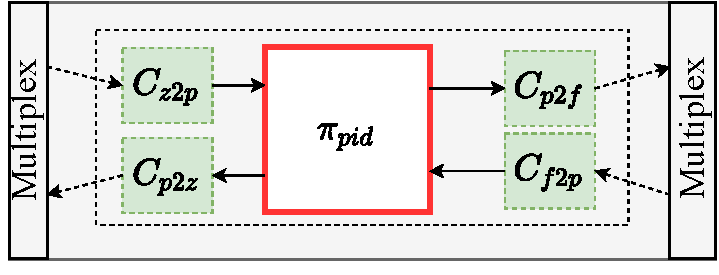
\includegraphics[scale=0.5]{figures/singleshellmultiplex.pdf}
	\caption{This is the \partywrapper that routes messages to the correct internally runnint protocol party. This figure shows how one protoco party (dotted box) is instantiated within it. The party $\pi_{pid}$ is shell code akin to Figure~\ref{fig:newpandq}.}%\snote{Updated caption to say it's multiplexer with one instance. The reason I don't want to include another instance is that I couldn't figure out a way to add it and expand the diagram horizontally. It will leave so much white space on the sides if I add a new party and will take up much more vertical space which we need to cut down on anyway.}}
	\label{fig:singlemultiplex}
	\vspace{-3mm}
\end{figure}
The \partywrapper spawns protocol parties, runs them in a sandbox, and routes messages to/from them and \Z, \F, and \A.
As a result of using channels, NomosUC needs the \partywrapper to handle spwaning new parties, the channels they require, and connecting them to the rest of the experiment.
%Without the \partywrapper, NomosUC may have to rely on \Z to create the channels for new parties and route messages to them.
%Similarly, \F and \A would have to all handle new channels from the creation of new parties.
%The \partywrapper runs all of the protocol parties internally in a sandbox, has one providerless channel to \Z, one to \A, and one with \F, and it multiplexes messages to and from them to its internal parties. 
%The \partywrapper is not a requirement specific to the session-typed setting of NomosUC, but motivated by the use of channels for communication.

The sandboxed parties communicate over virtual providerless channels, using a virtual token type, with the \partywrapper, but see an interface that's directly connected to \F or \Z. 
The \partywrapper connects to \F, \A, and \Z through communicators and multiplexes incoming and outgoing messages by the $\m{PID}$ included in them. 
We depict a single, sandboxed party running inside the \partywrapper in Figure ~\ref{fig:singlemultiplex}.
It is important to note that like most providerless channels, the construction of channels here is protocols/functionality-dependent---they must convert between message types and offer the correct session types. 
Typically, such protocol-specific communication constructs are written by users, as is the case with EasyUC~\cite{easyuc}, but in NomosUC the constructions are so trivial and can be systematically generated based on the type and PID of the party.

%In actuality, the \partywrapper is connected to \Z via communicator whose type includes the $\m{PID}$ with every message, and it routes messages to the appropriate virtual instance.
%An example of a party $\pi_i$ running within the \partywrapper is shown in Figure~\ref{fig:singlemultiplex}. The process $\pi_{pid}$ is the shell process mentioned previously and is connected to communicators as expected from providerless channels. The endpoint of the communicators is the \partywrapper.  

The \partywrapper construction trades off dynamic parties with expressiveness of import in session types.
All messages between \Z and protocol partis, for example, pass through the same providerless channel with the \partywrapper, and, therefore, only allows a static amount of import to be passed in each direction.
Tight runtime constraints, however, are not intended goals of NomosUC or the UC framework.

%\paragraph{Functionality Shells}
%As a consequence of our design, the \partywrapper construction must extend to \F as well.
%Instead of losing the soul of session types that we're pursuing, we replicate the virtualization of the \partywrapper for functionalities to meaningfully use session types. 
%NomosUC runs \F in a shell and communcates with \A and the \partywrapper through providerless channels. 
%The same reasoning about the impact of import in the \partywrapper applies here.
For the remainder of this work we denote and individual protocol party as $\pi$ or $\pi_i$, and a protocol as a whole run inside the \partywrapper as $\m{MX}(\Pi)$ or $\m{MX}(\pi)$.

% important things to mention here:
%   -- ideal functionalities do the same thing as the multiplexer and have to create extra processes to parameterize them with channels
%   -- constraints on session types that arises from some functionalities 
\subsection{Ideal Functionalities}
The core of the UC framework is the ideal functionality: it captures the desired security properties and defines the protocol interface as a simple trusted third party. 
Its session types with parties contrains the order of messages and import required, it provides the user insight into the functionality and its interface, and succintly captures the protocol's state machine.
Like the \partywrapper, we must treat functionalities as being wrapped by code that communicates with the other processes, and the wrapper around a functionalities creates the same dummy processes that offer the desired session types. 

Supporting a dynamic number of parties at the ideal functionality has its own challenges unique from the \partywrapper.
For example, the code of a functionality can only wait to read (a blocking operation) on a static number of channels defined in the process code. 
In some case, \Fauth overcomes this obstacle by implementing the simpler one-way functionality \Fsmc and applying the multisession operator described later in this section. 
Others resort to a polling-based approach where parties query the functionality for new messages or output to be delivered.

%Linear session types require some tradeoff when definin them for ideal functionalities, and we highlight them through the 2-way communiation channel \Fauth.
%
%\Fauth accepts messages from two parties and allows \A to decide when the message is delivered to the other.
%At a given moment, party $P_i$ can give input to, or expect output from, \Fauth. This implies a session type must both accept internal choice and external choice at the same time---a pattern that can not be realized.
%In such cases, we sacrifice some of the expressiveness of session types and resort to splitting communication between two uni-direcitonal channels.
%We show this type for \Fauth below. 
%%From the point of view of either part $P_i$, it can write to \Fauth or receive a message from it---a communication pattern that can't be expressed by a single session type.
%%Most functionalities that exhibit ambiguity in which end point can send a message must fallback on two competing approaches: split communication over two uni-directional channels or switch communication to polling where the party or \A asks \Fauth for new messages.
%%Both cases can be captured by session types but lose some of the power of the session type mediating the order of messages in the protocol. 
%%For example int he former approach the session types for \Fauth look something like this
%
%%We use providerless channels, in part, to allow functionalities in NomosUC to use meaningful session types with a dynamic number of parties.
%%The 2-way channel ideal functionality, \Fauth, is a simple and clear illustration of design choices and tradeoffs when writing functionalities in NomosUC.
%%\Fauth provides only message \emph{integrity} and leaks the message to \A.
%%When a message is sent by $P_s$, \Fauth sends the message to \A and waits for a response to deliver it to $P_r$. 
%%
%%In plain session types, communication between two parties $P_s$ and $P_r$ occurs over a single duplex channel.
%%In UC the role of the adversary as a message scheduler in \Fauth, the most common network channel model, means a more complicated functionality involving $P_s$, $P_r$, \F, and \A. 
%%\Fauth provides only the following guarantee: (\emph{integrity}) the adversary can not modify messages from the sender.
%%It sends the message to \A when it receives one from the sender, and waits for the adversary to instruct it to deliver the message.
%%When \A writes back to \Fauth to deliver the message, \Fauth sends it to the receiver.
%%The communication pattern in \Fauth exhibits the same problems with the communication in Figure~\ref{fig:newpandq}.
%%
%%We, therefore, are confronted with two options: transition to a functionality where all parties and the adversary poll for new messages or split communication among two uni-directional providerless channels.
%%The former buffers messages from $P_s$ until asked for by $A$, and then delivers (with \A's approval) to $P_r$ when polled.
%%The type and mechanics of this version require constant activations by \Z and are inconvenient.
%%The latter is a more generalizable construction and can be typed as: 
%\begin{center}
%\parbox{0cm}{
%\begin{tabbing}
%$\m{sendmsg}[a] = \textcolor{red}{\getpot^n} \ichoice{\mb{send}: \m{a} \product \m{sendmsg}}$ \\
%$\m{recvmsg}[a] = \textcolor{red}{\getpot^m} \echoice{\mb{recv}: \m{a} \product \m{recvmsg}}$ \\
%$\m{adv}[a] = \echoice{\mb{leakmsg}: a \product \ichoice{ \mb{ok}: \m{adv}}}$
%\end{tabbing}}
%\end{center}
%We can recover some expressiveness by making use of polymorphism in our types. In this example the session types are parameterized by a type \inline{a}. 
%\Fauth parameterized by channels using the ambiguous \inline{a}, makes it impossible for \Fauth to typecheck unless a \mb{recv} with before a \mb{send} that concretizes \inline{a}.
%The protocols concretize polymorphic functionalities, and, in general, we can use this trick anywhere we split communication into two-unidirectional channels to enforce ordering of messages between channels. 
%We show a more complicated, but contrived, example in Section~\ref{sec:functionalities} which expandds on how this trick can be used. 

%Supporting a dynamic number of parties also comes with limitations on expressiveness. 
%For example, NomosUC code can only wait for messages on a static number of channels because read operations are blocking. 
%Some functionalities, like p2p message passing between an arbitrary number of parties, don't share state between pairs of parties and can be implemented by defining simpler functionalities, like a one-way channel, and applying a generic opertor like the multisession defined later in this section.
%For others, we resort messages polling approaches where the functionality can ask each channel for new messages and react when given one. 
%This tradeoff also comes up in some functionalities that do not exhibit this communication pattern, but handle a dynamic number of parties without a communication pattern like \Fro described in a later
%With \Fro, we can use the same channel for every party because of the type of the communication, however, in general the code of a functionaliy can only \emph{wait} on a statically defined number of channels at a given moment. Therefore, in such cases, we also split the channels and use polymorphism to maintain ordering.
%where each party has one channel typed as $\m{sending}$ and the other as $\m{recvmsg}$.
%Despite this limitation we note that the type parameter $a$ for the message type ensures that no party can receice a message from \Fauth before a message is sent which concretizes $a$ to some type.
%Therefore, although some of the power of session types is lost when dealing with such functionalities, they are still capable of enforcing protocol message ordering and providing resource analysis through import.

\subsection{Polynomial Bound}
The UC framework introduces the concept of import tokens as a new way to reason about ITMs being polynomial in the security parameter $k$. 
The import mechainsm as described in UC, and which we describe in Section~\ref{sec:background}, ensures that a single ITM's execution is upper-bounded by some poynomial $T(n,k)$ where $T$ is a polynomial, $n$ is its net import token balance (received - sent), and $k$ is the security parameter.

In Section~\ref{sec:import}, we described how the NomosUC type systems judges processes to be PPT in the security parameter $k$. 
It still remains to show that our definition is sound by extending the arguing that the UC experiment \m{execUC} is polynomial time.
\begin{ddef}[PPT in $k$]\label{def:ppt}
A closed term $e(k,r)$ is  PPT in $k$ if, given some amount of initial import $n \in poly(k)$, there exists a polynomial $T(n,k)$ such that $\forall k, r, e(r,k) \{n\}$ terminates in at most $T(n,k)$ steps.
We use the notation $e(r,k) \leq T(n,k)$ to refer to such a PPT process.
\end{ddef}
%Notice that our choice of polynomial representation, a function of both the import and security parameter $k$, only partially defines PPT in terms of the security parameter. It still remains to be shown that the system is polynomial \emph{only} in $k$.

Soundness is a simple argument to make and comes down to showing that our UC experiment is PPT in only the security parameter $k$. 
%The UC framework provides a simulation of a configuration of ITMs on a universal turing machine and proves that such a turing machine is also bounded by a polynomial $T$. 
%Given the initial input of import tokens into the machine ($poly(k)$ amount of import), it concludes that the import mechanism falls in line with the standard length-of-input notion of polynomial time and satisfied their ``PPT in $k$'' definition. 
In NomosUC, we do not deal directly with ITMs, however, our type system allows us to judge whether a process, or collection of processes through the Preservation Theorem~\ref{thm:preservation}, is locally PPT given a particular polynomial. 
We rely on the Lemma~\ref{lem:local_ppt} and Theorem~\ref{thm:global_ppt} to adapt Proposition 7 from UC~\cite{canettiUC} to NomosUC, and show that our notion of locally PPT leads to a UC execution that is PPT in the security parameter $k$.

%In order to reason about configurations in Theorem~\ref{thm:soundness}, we define the UC execution as a series of configurations that capture the relevant processes--the \partywrapper, \Z, \F, and \A--and the channels that connect them.
\begin{theorem} \label{thm:soundness}
Let \F, \A, \Z, and \m{MX}(\PI) be locally PPT configurations bounded by super additive polynomials $T_\F$, $T_\A$, $T_\Z$, $T_\PI$. Let \m{UC} be a configuration composed of a single process that runs \inline{execUC}. If \m{UC} receives $n \in poly(k)$ import initially, then any composed configuration $\m{UC} = \m{execUC} \; || \; \Z \; || \; \A \; || \; \m{MX}(\PI) \; || \; \F$ is PPT in $k$, where \m{MX} is the \partywrapper.
\end{theorem}

\begin{proof}
It suffices to argue that the resuting process configuration \m{UC} offers only one channel, the one offered by \m{execUC}.
As $n \in poly(k)$ is the total import given to \m{UC}, and by Lemma \ref{lem:local_ppt} and Theorem \ref{thm:global_ppt}, we can conclude that $\m{UC} \leq poly(k)$.
\end{proof}
\todo{@Andrew: we had a discussion that such a theorem as is necessary, but with the global PPT theorem and proof in the type system section is it really necessary? we're just relying on those two lemmas so what's the point.}

\subsection{Emulation}
The central security definition in UC is indistinguishability between the real and ideal world experiments.
In NomosUC, we define the term \textit{well-matched} to mean the configuration resulting from a PPT term $e$ connected to another term $e'$ in well-typed, and we denote it as: $e \leftrightarrow e'$.
The term allows us to quantify statements over only adversaries and environments whose types match the protocol/functionality in question when reasoning about emulation. 

We define the output bit of the partial term of \inline{execUC}, for a specific $\pi$ and \F, as an ensemble of distributions over all possible random bitstrings and security parameters.
Emulation, then, is about the ensembles created by two UC executions being computationally indistinguishable from each other.
We define indistinuishability between ensembles in a standard way using \textit{statistical distance}: $\mathcal{D}_{1,k} sim \mathcal{D}_{2,k}$ if their statistical distance is at most $negl{k}, \forall k$.
%\begin{definition}[Indistinguishability]\label{def:distance}
%Two ensembles $\mathcal{D}_{1,k}, \mathcal{D}_{2,k}$ are indistinguishable, $\mathcal{D}_{1,k} \sim \mathcal{D}_{2,k}$, if their statistical distance is at most $negl(k), \forall k$.
%\end{definition}

UC emulation combines the UC execution with indistinguishability resulting in the following NomosUC emulation definition.
\begin{definition}[Emulation]\label{def:emulation}
If two protocols $(\pi, \F_1)$, $(\phi, \F_2)$, which we refer to only by \PI and $\phi$, emulated each other, then $\forall \A$ well-matched with \PI, there must $\exists \Sim$ well-matched with $\phi$ s.t. $\forall \Z$ : $\msf{execUC}(\pi, \F_1, \Z, \A)$ $\approx$ $\msf{execUC}(\phi, \F_2, \Z, \Sim)$:

\begin{mathpar}
	\footnotesize
	\inferrule*[right=emulate]
	{
		\pi : \Delta_1'[\Tokentypes][\mathrm{T}_{\pi}] \semi \phi : \Delta_2'[\Tokentypes][\mathrm{T}_{\phi}] \semi \\
		\forall \A \ | \ \Delta_4[\Tokentypes][\mathrm{T}_{\A}] \vdash \A :: \Delta_3', \ \langle \A \leftrightarrow \pi \rangle \\
		\Rightarrow \exists \ (\Delta_3[\Tokentypes][\mathrm{T}_{\Sim}] \vdash \Sim_\A :: \Delta_3') \ | \ \langle \Sim_\A \leftrightarrow \phi \rangle \\
		\Rightarrow \forall \Z  \; \msf{execUC} \ \pi\ \Z\ \F_1\ \A \approx\ \msf{execUC} \ \phi\ \Z\ \F_2\ \Sim_\A
	}
	{
		% EMULATION DEFINITION
		\lambda \A \, . \, \Sim_\A \vdash (\pi, \F_1) \sim (\phi, \F_2)
	}
\end{mathpar}
\end{definition}

An important validation of our approach is the the Dummy Lemma~\ref{thm:dummythicclemma} which shows that a simulator for the dummy adversary satisfies the emulation definition for all adversaries. The proof of the Lemma is a simulator that we state in Appendix Section~\ref{sec:diummy}, but we sate the theorem here. 
\begin{theorem}[Dummy Lemma]\label{thm:dummythicclemma}
If \ $\exists \DS$ s.t. $ \DA, \DS \vdash \F_2 \xrightarrow{\pi} \F_1$ then $\forall \A \ \exists \Sim_\A$ s.t. $\Sim_{\A} \vdash  \F_2 \xrightarrow{\pi} \F_1)$ 
\end{theorem}

\subsection{Single Composition}
In this section we present a composition operator for protocols that completes the single composition theorem, Theorem~\ref{thm:singlecomp}.
The composition operator allows replacement of a functioality with a protocol realizing it, and, potentially, any functionality that protocol uses.

In NomosUC, composition of protocols occurs in the \partywrapper where output from $\rho_i$ to $\F_2$ is given as input to $(\pi, \F_1)$. $\pi$ runs in the \partywrapper and $\F_1$ is the hybrid functionality. 
The generic composition operator of NomosUC connects the shells of parties $\rho_i$ and $\pi_i$ through providerless channels. 
As mentioned earlier, for functionalities/protocols that don't need to split communication over two channels, the coposition operator can be trivialized by directly connected the channel offered by $\rho_i$ as the input channel of $\pi_i$.
The type system here guarantees that our composition gives $\pi_i$ an appropriate amount of import and tha the resulting protocol is also polynomially bound. 

Part of the security proof of security under composition is providing a simulator that ensures emulation.
For this we can defina simulator compostion operator that connects the simulators \SIM{\rho} and \SIM{\pi} in the natural way. 
Inputs to the adversary are intended for $\F_1$ or dummy parties of $\F_1$ and are handled by \SIM{\pi}. Outputs from \SIM{\pi} are intended for $\F_2$ and dummy parties of $\F_2$ is simulated by \SIM{\rho}.

\subsection{UC Composition}

\begin{theorem}[Composition]\label{thm:composition}
\begin{mathpar}
\inferrule*[right=compose]
{
	%(\pi, !\F_1) \sim (\idealP, F_2) \semi (\rho, !\F_2) \sim (\idealP, \F_3) \\ 
	!\F_1 \xrightarrow{\pi} \F_2 \semi !\F_2 \xrightarrow{\rho} \F_3 \\
	%\Rightarrow \exists \Sim(\A) \vdash (\rho^{!\F_2 \rightarrow (!\pi \, \circ \, \msf{squash})}, !\F_1) \sim (\idealP, \F_3)
}
{
	!\F_1 \xrightarrow{\rho \, \circ !\pi \circ \, \msf{squash}} \F_3
	%(\rho \, \circ \, !\pi \circ \msf{squash}, !\F_1) \sim (\idealP, \F_3)
}
\end{mathpar}
\end{theorem}

Full composition in the UC framework extends beyond the simpler composition in Theorem~\ref{thm:singlecomp} allowing replacement of only one instance of a functionality with a protocol that realizes it.
Instead, UC composition allows for replacement of any number of instances of a functionality with instances of the realizing protocol.
Theorem~\ref{thm:composition} illustrates the full composition theorem using our arrow notation, and highlights a theorem that we must prove before we can achieve full composition.
%We rely on two sub-theorems that make use of the multisession extension: Theorem~\ref{thm:squash} and Theorem~\ref{thm:functor}.
We rely on a sub-theorem that makes use of the multisession extension: Theorem~\ref{thm:functor}.
\begin{theorem}[Multisession Composition]\label{thm:functor}
	\begin{mathpar}
		\inferrule*[right=MultiComp]
		{
			\F_1 \xrightarrow{\pi} \F_2
		}
		{
			!\F_1 \xrightarrow{!\pi} !\F_2
		}
	\end{mathpar}
\end{theorem}
The detailed description of this extension and its security proof can be found in the Appendix. At a high level is shows that security holds when protocols/functionalities are arbitrary replicated and run concurrently.
We also prove an adjacent Theorem~\ref{thm:squash}, in the appendix, which allows squashing a doubly-applies multi-session extension to a single application of it with a \msf{squash} protocol ($!!\F \xrightarrow{\msf{squash}} !\F)$.

Defining these extensions, theorem and their simulators in NomosUC allows us to conclude that NomosUC captures the full, generlized UC composition theorem with the following argument. 

\begin{proof}
By Theorem~\ref{thm:singlecomp} we have that $\F_1 \xrightarrow{\pi} \F_2$. If we combine this result with Theorem~\ref{thm:functor} we can conclude that $!!\F_1 \xrightarrow{\rho \circ !\pi} !\F_3$. 
Finally we can squash one $!$ operator with Theorem~\ref{thm:squash} (in Appendix~\ref{app:ms}) to get $!\F_1 \xrightarrow{\rho \circ !\pi \circ \m{squash}} \F_3$.
\end{proof}


